%%%%%%%%%%%%%%%%%%%%%%%%%%
% USFD Academic Report Template
% Prof. Roger K. Moore
% University of Sheffield
% 30 July 2018
%%%%%%%%%%%%%%%%%%%%%%%%%%


\documentclass[11pt,oneside]{book}
\usepackage[margin=1.2in]{geometry}
\usepackage[toc,page]{appendix}
\usepackage{graphicx}
\usepackage{lipsum}
\usepackage{caption}
\usepackage{cite}
\usepackage{url}
\usepackage{array}
\usepackage{longtable}
\usepackage{amsmath} 
\usepackage{tocloft}
\usepackage{float}

\setlength{\parskip}{1em}
\setlength{\parindent}{0pt}
\setlength{\cftbeforesecskip}{0.5em}

% Set row padding for all tables
\renewcommand{\arraystretch}{1.2}

\begin{document}

\captionsetup[figure]{margin=1.5cm,font=small,labelfont={bf},name={Figure},labelsep=colon,textfont={it}}
\captionsetup[table]{margin=1.5cm,font=small,labelfont={bf},name={Table},labelsep=colon,textfont={it}}
\setlipsumdefault{1}

\frontmatter

%TC:ignore
\begin{titlepage}

\begin{center}
{\LARGE University of Sheffield}\\[1cm]
{\Large COM3610 Dissertation Project}\\
\linespread{1.2}\huge {\bfseries Automating Fantasy Football: Leveraging Machine Learning for Predictive Analysis and Squad Optimization}\\[1.5cm]
\linespread{1}

\includegraphics[width=4cm]{images/UOSLogo.png}\\[1cm]
{\Large Ian Vexler Galarza}\\[1cm]
{\large \emph{Supervisor:} Phil McMinn}\\[1cm] % if applicable
\large A report submitted in partial fulfilment of the requirements\\ for the degree of BEng Software Engineering by Ian Vexler Galarza\\[0.3cm] 
\textit{in the}\\[0.3cm]
Department of Computer Science\\[2cm]
\today
\end{center}

\end{titlepage}


% -------------------------------------------------------------------
% Declaration
% -------------------------------------------------------------------

\newpage
\section*{\Large Declaration}

All sentences or passages quoted in this document from other people's work have been specifically acknowledged by clear cross-referencing to author, work, and page(s). Any illustrations that are not the work of the author of this report have been used with the explicit permission of the originator and are specifically acknowledged. Additionally, generative AI tools, such as ChatGPT, have been utilized to improve the clarity and quality of the text. All usage of such tools has been limited to language refinement and no content generated has been presented as original research or analysis. Examples of prompts used are included in Appendix A. I understand that failure to attribute sources amounts to plagiarism and will be considered grounds for failure.\\[1cm]

\noindent Name: Ian Vexler Galarza\\[1mm]
\rule[1em]{25em}{0.5pt}

% \noindent Signature:\\[1mm]
% \rule[1em]{25em}{0.5pt}

\noindent Date: 08/12/2024\\[1mm]
\rule[1em]{25em}{0.5pt}


% -------------------------------------------------------------------
% Abstract
% -------------------------------------------------------------------

\chapter*{\Large \center Abstract}

% One or two sentences providing a basic introduction to the field, comprehensible to a scientist in any discipline.  Two to three sentences of more detailed background, comprehensible to scientists in related disciplines.  One sentence clearly stating the general problem being addressed by this particular study.  One sentence summarising the main result (with the words ``here I show'' or their equivalent).  Two or three sentences explaining what the main result reveals in direct comparison to what was thought to be the case previously, or how the main result adds to previous knowledge.  One or two sentences to put the results into a more general context.  Two or three sentences to provide a broader perspective, readily comprehensible to a scientist in any discipline.

Fantasy Premier League (FPL) is a globally popular game that combines strategic gameplay with real-world football performances. The complexity of FPL, which includes player selections, transfers, and strategic chip usage, makes it ideal to benefit from a data-driven approach to obtain a competitive advantage. This can be done by applying advanced predictive and optimisation techniques.

This report explores the development of a machine learning-based system to optimise FPL performance. The project aims to demonstrate the effectiveness of these methods through a multi-stream analysis tailored to player positions. The system's performance is evaluated through a comparison of multiple strategies, including both purely data-driven methods and approaches inspired by top-performing FPL managers, looking to find the optimal approach.

Through this work, the project demonstrates how artificial intelligence and statistical analysis can address challenges in data integration, temporal dependency modelling, and strategy optimization.


% -------------------------------------------------------------------
% Contents, list of figures, list of tables
% -------------------------------------------------------------------

\clearpage
\tableofcontents

% \clearpage
% \listoffigures

\clearpage
\listoftables


% -------------------------------------------------------------------
% Main sections (as required)
% -------------------------------------------------------------------
%TC:endignore

\mainmatter

\chapter{Introduction}

\section{Background}

Fantasy Premier League (FPL) has become a popular pastime for millions of football fans, combining the excitement of live sports with strategic gameplay. Initially introduced for the 2002/03 season, FPL is the most popular Fantasy Football game globally, with over 11 million users as of 2024 \cite{fpl}. Users build teams consisting of real-life players, earning points based on their performances in real matches.

As competition becomes increasingly challenging, effective strategies and data-driven decisions has never been more important. FPL's complexity goes beyond selecting players and lining them up in a team, the game offers users the chance to perform transfers and use chips strategically to increase their chances of winning. Due to this, leveraging machine learning and optimisation techniques could be key to improving performance.

\section{Aims and Objectives}

This project aims to develop a machine learning system capable of performing among the top players in FPL. By leveraging historical data, predictive models and optimization strategies the system aims to optimise team management and overall performance in the game. The ultimate goal is demonstrating that these tools can achieve a competitive advantage.

To achieve this aim, the project will pursue the following objectives:

\subsection{Collect and preprocess historical FPL and football data}

The data collection process includes player performance metrics, fixture schedules and other contextual information required for predictive modelling.

\subsection{Player performance predictor}

The ability to simulate a season is required to fully automate FPL. The overall aim is to leverage regression analysis to predict how each player will perform through each Gameweek in a season. This project will compare different techniques and use careful feature selection to find the optimal model for performance predictions.

\subsection{Team selection}

Given that the FPL dataset contains hundreds of players and many valid formations, the project will look at implementing optimisation algorithms to select the best possible combination. In addition, transfers  between Gameweek, can add more complexity to this challenge.
% Maybe mention injuries?

\subsection{Captain and Chip usage}

FPL offers the chance to boost results further by captaining players or utilising different chips. This project will analyse the most efficient strategies to use these and apply them during automation.

\subsection{Evaluate the performance}

To assess the quality of the results, the project will evaluate the system against different baselines and compare the performance of different strategies to find the optimal.
\chapter{Literature Survey}

In recent years, data analysis and machine learning have transformed Fantasy Premier League, allowing managers to make more informed decisions and have greater success in their strategies.  This chapter begins with an overview of the rules and constraints of FPL, setting a foundation for automated strategies. The review then explores previous research on predictive modelling, relevant strategies and optimisation techniques. Finally, the chapter expands on the models to be used and their application in the context of this project.

\section{Fantasy Premier League: rules and constraints}

FPL rules define the game and add layers of complexity. From budget and transfer restrictions to squad selection, the rules shape strategy. These constraints force users to adapt and plan for short-term and long-term outcomes causing them to make crucial decisions under uncertainty.

This section explores the fundamental rules and constraints of FPL, demonstrating how they affect possible outcomes. By understanding these, we can better appreciate the problem FPL automation faces and the obstacles it must overcome. The complete FPL rule set is publicly available at the official FPL website \cite{fpl}.

\subsection{Team selection and management}

Users must select a squad of real-life players. This squad must consist of:
\begin{itemize}
    \item 2 Goalkeepers
    \item 5 Defenders
    \item 5 Midfielders
    \item 3 Forwards
\end{itemize}

In addition, these must fall within a strict budget of £100 million, and no more than three players from each team must be selected. Hence, a careful and optimised selection is needed.

Each Gameweek, managers select 11 starters, with the remaining 4 benched. If one or more of the selected do not play, the system automatically substitutes them based on the bench order. Players are also restricted to choosing between 8 formations, requiring at least one goalkeeper, three defenders and one forward.

\subsection{Captain and Vice-captain}

From the starting 11, one can select a captain and vice-captain. The game awards the captain double the number of points. If the captain does not feature during a Gameweek, the vice-captain will receive the points.

\subsection{Transfers}

Transfers allow managers to buy and sell players after forming their initial squad. One free transfer is granted each Gameweek, which can be accumulated for up to five tokens (or two until the 2024/25 season). A four point penalty is given if any additional transfers are performed. Depending on their popularity in the transfer market, player prices change dynamically during a season.

\subsection{Chips}

Each Gameweek, chips can be used to improve performance further. Users are restricted to only one chip per Gameweek. The Chips available are:
\begin{itemize}
    \item \textbf{Bench Boost}: The points obtained by benched players also count toward the total score.
    \item \textbf{Free Hit}: The user can make unlimited free transfers for a single Gameweek. After that, the team returns to the state before applying the chip. 
    \item \textbf{Triple Captain}: The selected captain's points are tripled instead of doubled.
    \item \textbf{Wildcard}: Allows to perform unlimited permanent transfers free of charge. Available twice a season. 
    \item \textbf{Mystery Chip}: Only available from January 2025, unknown when writing this.
\end{itemize}

\subsection{Points system}

% TODO: Reference table
Players are allocated points according to their performance in real life. Table~\ref{tab:fpl_points} presents how players can earn these.

\begin{longtable}{|>{\raggedright\arraybackslash}p{10cm}|c|}
\hline
\textbf{Action} & \textbf{Points} \\
\hline
For playing up to 60 minutes & 1 \\
\hline
For playing 60 minutes or more (excluding stoppage time) & 2 \\
\hline
For each goal scored by a goalkeeper & 10 \\
\hline
For each goal scored by a defender & 6 \\
\hline
For each goal scored by a midfielder & 5 \\
\hline
For each goal scored by a forward & 4 \\
\hline
For each goal assist & 3 \\
\hline
For a clean sheet by a goalkeeper or defender & 4 \\
\hline
For a clean sheet by a midfielder & 1 \\
\hline
For every 3 shots saved by a goalkeeper & 1 \\
\hline
For each penalty save & 5 \\
\hline
For each penalty miss & -2 \\
\hline
Bonus points for the best players in a match & 1-3 \\
\hline
For every 2 goals conceded by a goalkeeper or defender & -1 \\
\hline
For each yellow card & -1 \\
\hline
For each red card & -3 \\
\hline
For each own goal & -2 \\
\hline
\caption{Fantasy Premier League Points System \cite{fpl}}\label{tab:fpl_points} \\
\end{longtable}

\subsection{Conclusion}

FPL's rules create an environment where managers must balance budget limits, squad selection and transfer restrictions. These challenges make success in FPL a complex optimisation task, requiring a careful combination of short and long-term planning. Now that we understand the rules in detail, we can look at some of the strategies used by top-performing managers. These strategies show ways to tackle the game’s challenges and provide valuable insights that could be replicated when automating FPL.

% TODO
% Players can also be awarded Bonus Points (BPS)

\section{Popular FPL strategies}

To perform amongst the top FPL players, one could first learn from them and their approaches. This section will highlight some of their differential strategies that could be translated into our current objectives.

\subsection{Data-Driven Success}

In the 2023/24 season, Jonas Sand Labakk became champion, attributing his success to a data-driven approach. Labakk heavily relied on analytics, utilising expected statistics to make informed player and captaincy selections. His method involved planning up to six Gameweeks ahead, allowing for well-informed decisions and minimising bias in judgment. Labakk explained, "Human decision-making can, however, be biased, and an analytical approach allows me to spot players I would otherwise miss." \cite{fantasyfootballhub_labakk_2024}.

Labakk's strategy was focused on making decisions that minimised risk overall. For example, he favoured consistency when captaining over high-risk options. After an initial run of disappointing results, he went against popular trends to stabilise his team by adapting his chip usage and activating his Wildcard earlier than planned. Moreover, his usage of chips such as the Free Hit and Bench Boost was carefully timed to maximise point return, demonstrating his ability to balance low-risk decisions with opportunities for high returns \cite{premierleague_labakk_2024}.

Labakk's approach highlights the importance of data-driven decisions and careful planning, acting as an example of effective FPL management.

\subsection{First team selection}

Ali Jahangirov, the 2022/23 FPL season winner, shared some of the key strategies behind his success in a series of articles published on the Premier League website. 

When selecting his initial team, Jahangirov emphasised the role that flexibility and strategic planning played in his choices. He advised on having a balanced approach by investing in only two "premium" players, typically identified by their high cost and ownership rates. This strategy helps ensure the squad remains adaptable due to the high uncertainty in the season's early stages. Jahangirov also stressed the importance of analysing the upcoming fixture schedule, suggesting that managers should target players with favourable early fixtures \cite{fpl_jahangirov2023}. To minimise risk further, he recommended paying attention to ownership trends, as these figures reflect the strategies adopted by most FPL managers \cite{fpl_jahangirov2023_budget}.

\subsection{Chip usage}

In the 2022/23 FPL season, champion Ali Jahangirov had a strategic approach to chip usage that contributed to his success. For example, he favoured a delayed deployment of the first Wildcard, utilising it in Gameweek 12. This decision allowed him to restructure his team based on previous player performances and fixture schedules. Contrasting Labakk, Jahangirov emphasised the importance of resisting early temptations to activate the Wildcard, suggesting that patience enables better planning and adaptation.

Additionally, Jahangirov saved other chips, such as the Bench Boost and Triple Captain, for double Gameweeks (where players have additional fixtures), aiming to capitalise on players having multiple fixtures within a single Gameweek for maximum point returns. The champion also adopted an unconventional strategy by not triple captaining Erling Haaland, something that 520,778 managers did. He instead opted to captain Marcus Rashford, arguing that midfielders have a higher ceiling, a risky approach that allowed him to maximise his chip usage.

His approach to the Free Hit chip was similarly focused on leveraging double Gameweeks, where the potential for higher points is greater. Rather than following the popular strategy of using the Free Hit during blank Gameweeks (where several players may not have fixtures), he preferred to save them. Instead, he opted to use the chip during double Gameweeks for the potential of a greater outcome. This strategy complemented his use of the Bench Boost and Triple Captain chips, ensuring they were used during increased player activity \cite{fpl_jahangirov2023_chips}.

Jahangirov's calculated and patient strategy in chip deployment highlights the value of timing and informed decisions in FPL management. His approach serves as a baseline for optimising chip usage to get an advantage.

\subsection{Conclusion}

The strategies used by top FPL managers show how important data-driven decisions, planning and effective strategy are. From Labakk’s analytical and low-risk approach to Jahangirov’s emphasis on flexibility and optimised usage of chips, these methods highlight how one can tackle the complexities of FPL.

By studying these human strategies, we can get a solid foundation on techniques that can be used to optimise machine learning models. With this understanding, we now review how previous students tackled these challenges by exploring past projects focused on automating FPL.

\section{Past Dissertations}

Over the years, many students have attempted to address the challenges of automating Fantasy Premier League (FPL), producing a range of dissertations with varying levels of success. This section focuses on two of the most recent and notable projects, analysing their findings, methodologies and contributions to the field. By examining these works, this review aims to identifying gaps and opportunities for further research.

Pownall conducted a complete study on automating FPL management using machine learning techniques. His results showed that Linear Regression outperformed more advanced techniques like Ridge and Lasso regression, suggesting that simpler models could achieve good results on this task. Pownall then integrated these models with an optimisation framework, where he evaluated team selection strategies for maximizing total points. By simulating different transfer strategies and chip decisions, his dissertation provided insight into how predictive modelling could be used along with optimisation techniques to automate FPL. Finally, he evaluates the impact of external factors, such as injuries or managerial changes, on his predictions, highlighting the need for an adaptive system \cite{pownall2023fantasyfootball}.

Pownall's work, while providing a useful foundation, has some limitations. His choice to use simpler models, such as Linear Regression, might not be ideal for capturing complex relationships between player statistics and performance. Furthermore, he doesn’t seem to focus much on data preprocessing or feature engineering which could harm the predictive accuracy of the models. Finally, his analysis of external factors, while insightful, is mainly descriptive rather than integrated into the project, highlighting a challenge without offering a practical solution.

Tindal, adopted a different approach, focusing on other techniques to predict player performance and optimise team selection. His project evaluated the effectiveness of several models, including Linear Regression, Random Forest, Multi-Layer Perceptron (MLP) and Gradient Boosting, in predicting player performances, with the latter being the most effective. Tindal's work on feature engineering identified key statistics such as player form, fixture difficulty and team performance metrics, which appeared to have the highest impact on the results. His analysis showed that careful data preprocessing and feature selection played crucial roles when evaluating model performance. Additionally, his project mentions the challenges of missing key data and the approaches he used to mitigate this though some gaps remained unresolved \cite{tindal2023fantasyfootball}.

While Tindal’s work is valuable, it could be criticized for its focus on predictive accuracy without fully addressing the challenge of data scarcity. Additionally and in contrast with Pownall, Tindal’s analysis emphasizes feature engineering and the effects this has on predictive model accuracy. However, it does not explore in depth how these predictions could be used to experiment with and optimize different FPL strategies, such as team selection or chip usage. This gap provides an opportunity to investigate how predictive models can be combined with diverse strategic approaches in FPL management.

These dissertations provide invaluable insights and a strong foundation for this project. Tindal’s work highlights the importance of model selection and the role of feature engineering in improving predictive accuracy. Pownall’s research demonstrates the potential of integrating predictive modelling with optimisation strategies to manage a team effectively.

This dissertation aims to build on these projects and improve existing methods by exploring alternative machine learning models, feature engineering strategies and optimisation techniques. Additionally, this project aims to compare some of the regression techniques used in these studies, to determine the most effective approach.

By using their methodologies as a baseline, we aim to progress on of automated FPL management and evaluate how new approaches can improve upon their findings. While the results from these studies are promising, it remains important to explore if alternative models could be better suited for this task.

\section{Other Relevant Works}

Researchers have made many attempts to automate Fantasy Football with varying levels of success. As a well-explored area, we can learn from previous works to make this project successful.

\subsection{Innovative Regression Approaches}

Taking a more innovative approach, Ramdas \cite{ramdas2023cnn} explores the use of Convolutional Neural Networks (CNNs) to predict player performance. Traditionally used in image and video analysis, CNNs prove to be surprisingly effective in this context, outperforming traditional regression models across all metrics. However, challenges remain, including the lack of publicly available spatio-temporal data in football and the significant preprocessing effort required for CNNs.

\subsection{Multi-stream Analysis}

Research has been conducted to enhance prediction accuracy by using multi-stream analytics models. For instance, Bonello compares statistical models with multi-stream models, where each stream represents a different position in the team. The results were mixed: while goalkeepers performed poorly under the multi-stream approach, forwards outperformed \cite{BonelloNicholas2019MDAf}. The findings can be explained by how different positions rely on team form versus individual skill. Similarly, Tindal applied a multi-stream approach with moderate success, arguing that positions have distinct scoring requirements \cite{tindal2023fantasyfootball}. A careful selection of features remains a key factor to achieve good results with this approach. By processing each position separately multi-stream models can better capture the characteristics of each, potentially improving the accuracy of player performance predictions.

\subsection{Leveraging Historical Data}

To address the limitations of traditional models, which lack temporal awareness, different approaches have been explored to represent player performance using both short-term and long-term features. In his study, Kotrba combines recent match statistics with aggregated averages from more extended periods, including the first half of the season and the last 5 or 10 games \cite{KotrbaVojtech2020Hifs}. This approach captures both immediate performance trends and season consistency. Similarly, research by Pownall represents player performance through accumulated statistics from the last five games, offering a perspective into recent form \cite{pownall2023fantasyfootball}. These adaptations make capturing temporal patterns in FPL predictions possible, where recent player performance can influence outcomes.

% TODO: Maybe?
Kristiansen introduced the idea of weighting long-term features to simulate temporal dependencies in FPL predictions better. His model incorporates factors such as opponent strength, player form and home advantage to adjust the weights of relevant statistics. By applying these weights, he aims to refine performance forecasting \cite{Kristiansen2024}.

\subsection{Temporal Dependency Modeling}

Adapting data to work with conventional machine learning models is a valid approach, but a more effective method may exist. Long Short-Term Memory (LSTM) Recurrent Neural Networks are particularly well-suited for handling sequential data such as natural language processing, speech recognition and time series forecasting \cite{jaff2023lstm}. These characteristics make them an excellent fit for this project as they can leverage the temporal dependencies in player Gameweek data, an advantage standard models lack.

LSTM networks were first applied to Fantasy Football predictions by Gupta, who noted that they effectively capture non-linear patterns without relying on linear components \cite{GuptaAkhil2019TSMf}. However, unlike more traditional models, LSTMs require a larger amount of data to capture these dependencies accurately, which can be a potential limitation for some datasets.

Further supporting the effectiveness of LSTMs, Lindberg and Söderberg  performed a comparison on a wide variety of popular models. LSTM networks outperformed other models in predicting player performance across all positions. Their results showed that LSTMs achieved the lowest mean squared error (MSE) in regression analysis, proving once again their strength in capturing complex time-dependent patterns \cite{lindberg2020comparison}.

\subsection{Team Selection}

To enhance team selection, it is essential to ensure that the chosen team has a broad range of player costs, as research on team diversity has shown. In his study, Gullholm emphasises the role of player cost diversity as a critical factor in building successful teams. He observes that player costs are often clustered, with approximately 33\% of players in a season sharing the same cost. When analysing the best-performing teams, he finds that 72\% fall into what he defines as "diverse" teams, meaning their player costs are more widely distributed. Gullholm suggests that this diversity may be directly linked to having players who contribute across multiple statistics such as goals, assists and clean sheets rather than relying on a few high-cost "luxury" players. His findings identify cost diversity as a feature commonly associated with high-performing teams \cite{GullholmJosef2022DiKF}.

\subsection{Conclusion}

These studies highlight different techniques and approaches aimed at improving regression predictions. From innovative applications of CNNs to temporal models like LSTMs, these works show the importance and use of machine learning techniques. Additionally, methods such as multi-stream analytics, the use of historical data and strategic team selection show strategies that could further allow us to maximise points. 

\section{Machine Learning Models}

This project aims to implement some of these techniques while combining them with ideas highlighted in previous sections of this chapter. To implement these, we need a solid understanding of the mathematical principles behind machine learning models, which will be explained in this section. 

\subsection{Linear Regression}

Linear Regression is a simple yet effective statistical method for predicting a target variable \( Y \) based on input features \( X_1, \ldots, X_i \), assuming a linear relationship between them. Its simplicity makes it a popular choice. However, linear regression may struggle to capture complex, non-linear patterns, raising some concerns about its fit for this project. The prediction formula is:

\begin{equation}
    \hat{y} = \beta_0 + \sum_{i=1}^{p} \beta_i x_i,
\end{equation}

where \( \beta_0 \) is the intercept and \( \beta_i \) are the coefficients of the input features.


\subsection{Gradient Boosting}

Gradient Boosting is an ensemble method that constructs decision trees sequentially, with each new tree correcting errors made by its predecessors. \cite{BentejacCandice2021Acao}. Gradient Boosting is well-suited for capturing complex non-linear relationships in data, making it effective for regression tasks.

The prediction for Gradient Boosting is expressed as:

\begin{equation}
    \hat{y} = \sum_{m=1}^{M} \nu f_m(x),
\end{equation}

where \( f_m(x) \) is the \( m \)-th weak learner, \( \nu \) is the learning rate and \( M \) is the total number of learners. The residuals, which represent the errors, are calculated as:

\begin{equation}
    r_i = y_i - \hat{y}_i^{(m-1)},
\end{equation}

where \( r_i \) is the residual for observation \( i \).

\subsection{Random Forest}
Random Forest is another ensemble learning method that combines multiple decision trees to enhance predictive accuracy and reduce the risk of overfitting. Each tree is built using a random sample of training data and a random subset of features at each split, which reduces tree correlation and improves performance \cite{BentejacCandice2021Acao}.

For regression, the final prediction is obtained by averaging the outputs of all the trees:

\begin{equation} \hat{y} = \frac{1}{T} \sum_{t=1}^{T} \hat{y}_t, \end{equation}

where \( T \) is the total number of trees.

\subsection{Long Short-Term Memory (LSTM) Networks}
LSTM networks are a type of Recurrent Neural Network designed to model temporal dependencies in sequential data \cite{KALA2024569}, such as player Gameweek data. LSTM networks address both long and short-term dependencies using an architecture that includes memory cells and three types of gates: forget, input and output.

The forget gate in LSTM decides how much of the past information should be discarded, with its activation function:

\begin{equation}
    f_t = \sigma \left(W_f x_t + U_f y_{t-1} + b_f\right),
\end{equation}

where \( \sigma \) is the sigmoid function, \( W_f \) and \( U_f \) are weight matrices, and \( b_f \) is the bias. This process allows the LSTM to filter out irrelevant past information.

The input gate incorporates new input into the cell state. It calculates a candidate update \( c'_t \) using:

\begin{equation}
    c'_t = \tanh \left(W_c x_t + U_c y_{t-1} + b_c\right),
\end{equation}

and updates the cell state \( c_t \):

\begin{equation}
    c_t = f_t \cdot c_{t-1} + i_t \cdot c'_t,
\end{equation}

where \( i_t \) is the input gate activation.

Finally, the output gate generates the current output \( y_t \) by filtering the cell state:

\begin{equation}
    y_t = o_t \cdot \tanh(c_t),
\end{equation}

where \( o_t \) is the output gate activation. This mechanism allows LSTMs to balance long-term memory with new input.

\subsection{Conclusion}

This section has introduced the mathematical foundations of the machine learning models used in this project. Linear Regression offers a simple approach but may struggle when it comes to capturing the complexity of FPL data. Gradient Boosting and Random Forest introduce ensemble learning techniques and are better equipped to handle non-linear relationships. Meanwhile, Long Short-Term Memory (LSTM) networks stand out for their ability to model temporal dependencies, making them particularly well-suited for sequential data like Gameweek performances. Each model has strengths and limitations, and its performance will depend on the data and careful pre-processing.

\section{Conclusion}

This chapter has explored the key factors and approaches related to automating Fantasy Premier League. By understanding the game’s rules and constraints, we’ve gained a clear idea of the challenges that make FPL so complex. The strategies of top-performing managers offer valuable insights, serving as inspiration for developing automated solutions. Past dissertations and related works have shown the range of machine learning and optimisation techniques available, showcasing their strengths, limitations and potential. Finally, we introduced the mathematical foundations of the key models that will be part of this project.

These insights present a baseline on which to build an automated system. With this knowledge, we can lay the groundwork for a system capable of offering a competitive advantage in FPL.
% NOTES ON THIS CHAPTER:
% - UPDATE THE TENSE OF THE SECTIONS ONCE IMPLEMENTED
\chapter{Analysis}

This section investigates and analyses the machine learning and optimization techniques that will be employed throughout the project's development. By analysing historical data and real-time football statistics, and with the strategic use of chips, the aim is to create a reliable system for optimising FPL team selections.

\section{Datasets}

This project primarily uses publicly available data provided by the Premier League via its official API. For convenience, it uses the historical FPL data archive collected in Vaastav's popular GitHub repository \cite{vaastav_fantasy_2021}. This repository offers an organized dataset that spans multiple seasons, allowing for a historical analysis of player performance and game outcomes.

In addition to the Premier League data, it will look to incorporate the latest statistics from FBref \cite{fbref}, a widely recognized platform for football analytics. FBref tracks metrics from more than 140 football competitions around the world, obtained from the leading data provider OPTA. Data scrapers will be used to gather statistics, which facilitates the integration of these metrics into the project.

\section{Performance Prediction Models}

To predict player performance over the course of a season, a selection of machine learning models will be developed and evaluated. The models considered will include a variety of techniques, such as Linear Regression, Random Forests, Gradient Boosting and Long Short-Term Memory Recurrent Neural Networks. A comparative analysis will be performed to identify the most suitable model for this task. To ensure a fair comparison, all models will be trained and tested using the same features obtained from pre-processed historical data, ensuring compatibility across models. Feature selection will be based on a combination of correlation analysis and domain knowledge. This will ensure that only the most relevant features are used, aiming to minimize overfitting. 

% Additionally, regularization techniques such as Lasso and Ridge regression will be used to further reduce overfitting.

A multi-layered approach will be used to optimise performance prediction. Different models will be used for each player position, each incorporating a different variety of features. This will help identify the combination of features that maximizes prediction accuracy for each position. The models will leverage both season statistics and data from the most recent Gameweeks to capture relevant trends. Different window sizes for past Gameweeks will be tested to determine the optimal number, allowing the model to make the most informed predictions. 

Preprocessing steps such as feature scaling and selection will also be carefully analysed. Each preprocessing decision can influence accuracy, so these steps will be evaluated to ensure they improve rather than harm the results.

\section{Team Selection}

To maximize the total points in FPL, it is essential to make an optimised selection of players. This project will utilize a genetic algorithm for optimisation, ensuring that the player selection respects the game's strict rules. Various selection strategies will be tested, many of which are inspired by successful FPL managers and past winners. A comparative analysis of these strategies will be conducted to identify the most effective approach.

Transfers play a crucial role in team optimisation, as strategic changes after each match week can significantly impact overall performance. The transfer process will prioritise removing the player with the lowest expected points for the upcoming Gameweek, provided a replacement is available. Suitable replacements will be players expected to generate higher points while staying within the available budget. Additionally, factors such as the upcoming fixture schedule for transfer candidates will be considered, ensuring that transfers not only improve the team in the short term but also align with long-term goals.

\section{Chip Usage}
The optimal use of FPL chips plays a critical role in maximizing points over the season. This section discusses the strategies for utilizing each chip based on historical data and model analysis.

\subsection{Bench Boost}
The Bench Boost chip is most effective during double Gameweeks, where players have two fixtures and a higher chance of scoring points. The analysis will evaluate strategies such as combining it with the Wildcard to enhance squad depth versus using it independently.

\subsection{Free Hit}
The Free Hit chip will be analysed to compare its effectiveness in blank Gameweeks against double Gameweeks. The focus will be on evaluating the overall impact and point differences in each scenario to determine the optimal timing for its deployment.

\subsection{Triple Captain}
The Triple Captain chip is planned for use during double Gameweeks, where the selected player has a greater scoring opportunity. The analysis will involve comparing conservative strategies (e.g. captaining the predicted highest-scoring player) against riskier approaches (e.g. captaining a midfielder for a higher points ceiling).

\subsection{Wildcard}
The Wildcard chip offers flexibility for major squad changes. The analysis will explore scenarios such as using the Wildcard when the team falls significantly behind the optimal line-up for restructuring or saving it for later use in combination with the Bench Boost during double Gameweeks to maximize performance.

% \subsection{Mystery Chip}

% Only available from January 2025, unknown at the time of writing this.

\section{Performance Evaluation}

In order to select the optimal predictive model, we need to first decide on an approach to evaluate and compare model performance. In this project, the evaluation will focus on both accuracy and consistency.

A range of metrics will be used to assess accuracy in player performance forecasting. For the regression models, the primary metrics will be Mean Absolute Error (MAE) and Mean Squared Error (MSE). MAE provides an overall view of error magnitude, while MSE gives additional weight to larger errors. These metrics will allow for detailed comparisons across models, helping to determine if complex models offer an advantage and improve performance.

To fully automate FPL, various team selection strategies will be applied to each model's predictions. These strategies will simulate different approaches FPL managers might take when selecting players based on the model’s output. The cumulative results across the season will be recorded and then ranked, comparing each model’s effectiveness in building a high-performing team. To draw accurate conclusions, the simulations will be performed multiple times to minimize the influence of random chance on the results. 

To empirically evaluate the results, the outcomes will be compared to those of real managers, measuring their ability to replicate successful strategies. The project’s performance will also be benchmarked against the works of Tindal \cite{tindal2023fantasyfootball} and Pownall \cite{pownall2023fantasyfootball}, evaluating whether it builds upon and improves their methodologies. Total points scored will be used as the measurement of performance, providing a straightforward and objective metric for success.

\chapter{Progress}

This chapter outlines the initial progress achieved in the implementation of key components and algorithms that make this project. The work done so far serves as a strong foundation for the future stages of development and analysis. Specifically, progress has been made in three crucial areas: data handling, team optimisation and regression modelling.

\section{Data Loader}

The development of a reliable data loader is a fundamental component of this project, allowing the extraction of data from multiple sources. Central to this is the DataLoader class, a parent class designed to handle various datasets such as those from Vaastav and FBref. Each data source is processed through its own subclass, ensuring that data from different origins undergoes careful pre-processing to achieve compatibility.

\subsection{Vaastav Integration}

The integration of Vaastav’s dataset has proven straightforward, as its data is well-structured and already pre-processed. The dataset is stored in multiple files and in a variety of formats, each of which has different uses in the project.

\subsection{FBref Integration}

In contrast, importing data from FBref presents many challenges. Unlike Vaastav, FBref lacks extensive pre-processing and its naming conventions and notations differ significantly from FPL’s official dataset. To try and address this, the project utilises Soccerdata, a Python library that scrapes football data from a variety of popular platforms \cite{soccerdata}. An initial version of the FBref data loader has been implemented, featuring a function to scrape player data across Europe’s top five leagues for each Gameweek of a specified season.

However, matching player statistics between FBref and the FPL dataset remains a major challenge due to naming discrepancies. For instance, FBref lists Arsenal midfielder Jorginho under such a nickname, while the FPL dataset uses his full name, “Jorge Luiz Frello Filho”. Addressing this requires the implementation of a name-matching algorithm, potentially leveraging techniques such as string similarity to ensure accurate mapping of player statistics.

\subsection{Team Notation Discrepancies}

Another significant challenge is the variation in team notations across data sources. For example, Tottenham Hotspur is referred to as “Spurs” in FPL but uses its full name in FBref. To resolve this, a dictionary-based approach has been adopted, mapping all known aliases to a unified representation for each team. This ensures consistency and prevents data conflicts.

\subsection{Progress and Future Improvements}

While the foundational data loader infrastructure is operational, several enhancements are planned. These include:

\begin{itemize}
    \item \textbf{Name Matching}: Designing an algorithm to effectively match player names across datasets, addressing discrepancies in formats and naming conventions.
    \item \textbf{Error Handling and Validation}: Implementing checks to detect and resolve inconsistencies in the data, ensuring its quality and reliability for further analysis.
    \item \textbf{Incorporating Additional Sources}: Leveraging the wide variety of data sources available in the SoccerData library. For example, ClubElo provides historical ELO ratings of European football clubs dating back to the 1950s \cite{clubelo}. This source can be used to contextualize the difficulty of opponents faced by players, not only in England but also across domestic and continental competitions in Europe.
\end{itemize}

This architecture is the baseline of a robust data handling pipeline, ensuring high-quality inputs for the regression models and analysis in the other stages of the project.

\section{Optimal Team Selection}

A baseline algorithm has been implemented to identify the optimal team by leveraging a genetic optimisation approach. Although still under development, the algorithm aims to find the best possible combination of players that maximizes total points while strictly adhering to FPL rules. Future iterations will incorporate additional factors, such as player popularity and form, to enable the evaluation of alternative team selection strategies.

\section{Regression Algorithms}

The development of regression algorithms for player performance forecasting is in progress, with the main focus going towards implementing an LSTM neural network. The first version of this model is close to completion and is designed to predict an entire FPL season. The model employs a multi-stream approach, utilising separate models for each player's position. However, its effectiveness is yet to be seen, as evaluation methods are yet to be developed.

To support the implementation, a Feature Selector class has been designed to be used across all regression models. This class standardizes the selection of features specific to each position, ensuring consistency and enabling a single source of truth. Additionally, a Feature Scaler method is being developed to optimise predictions by scaling features appropriately. Currently, scaling is performed dynamically based on feature characteristics, but further changes are expected to improve performance and reliability.
% \chapter{Methodology}

\lipsum  % Replace with your text


\section{Requirements}

\lipsum  % Replace with your text


\section{Analysis}

\lipsum  % Replace with your text


\section{Design}

\lipsum  % Replace with your text


\section{Implementation}

\lipsum  % Replace with your text

% \chapter{Results}

\section{Experiment 1}

\lipsum  % Replace with your text


\section{Experiment 2}

\lipsum  % Replace with your text

% \chapter{Discussion}

\lipsum  % Replace with your text

\chapter{Conclusions}

This project explores the application of machine learning techniques to automate Fantasy Premier League and its potential use to maximise performance. With the use of historical data, predictive modelling, and optimisation algorithms this project aims to create a system capable of performing amongst the top players of FPL.

Long Short-Term Memory (LSTM) networks were selected for their ability to model temporal dependencies and will be tested with the expectation of outperforming traditional regression models when predicting player performance. A multi-stream approach was adopted to enhance system accuracy by tailoring predictions to specific player positions. Additionally, optimisation algorithms will be implemented to tackle team selection. Multiple selection strategies will be evaluated to identify the most effective approach, from statistical methods to strategies inspired by top-performing FPL managers.

The research shows the potential of machine learning on this topic, where predictive accuracy and adaptability can offer a competitive edge. While progress has been made in data preprocessing, model selection, and system implementation, challenges such as data integration and evaluation remain areas that need further development.

There are some limitations to this project that, while not critical, are worth mentioning. To properly evaluate the results, it will be necessary to run multiple simulations across different seasons and configurations, each with significant data requirements. This might require significant computational power, but the High-Performance Computing services at The University of Sheffield could help address this. Additionally, predicting the performance of new and young players presents a big challenge due to the lack of publicly available data. Multiple data sources will ideally be used to address this, but this approach carries risks. Ensuring the integrity of the data will require careful validation throughout the project.

This project establishes a solid foundation for FPL automation. By refining the predictive models and optimisation strategies, the system holds the potential to rival top-performing users. Figure~\ref{fig:gantt_chart} presents an overview of the general plan for the remaining time of the project, highlighting key deadlines.

\begin{figure}[H]
    \centering
    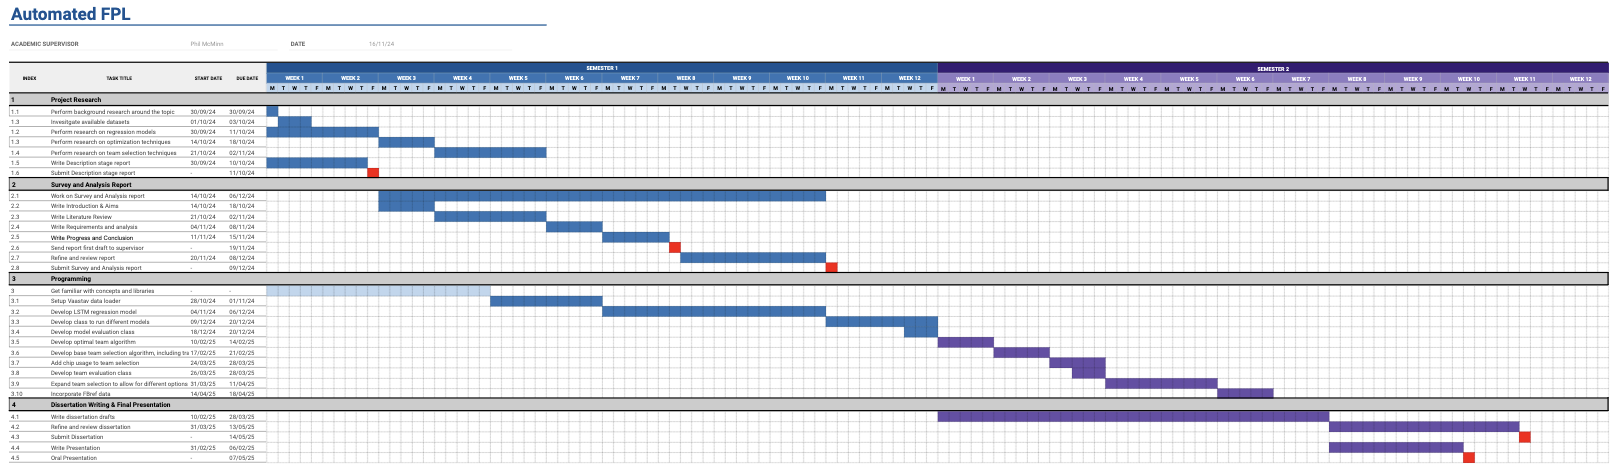
\includegraphics[width=15cm]{images/gant_chart.png}
    \caption{Overview of the project timeline}
    \label{fig:gantt_chart}
\end{figure}

Figure \ref{fig:gantt_chart} lays out a clear step-by-step breakdown of how each stage of the project will be tackled. There’s some uncertainty about how long it will take to implement the LSTM model, so extra time has been accommodated in case of any unexpected delays. Similarly, the expansion of team selection techniques has been planned for later in the project, with additional time allocated due to the unpredictability of how much time will be available to explore a wide range of methods. Finally, incorporating FBref data is considered a nice-to-have rather than a core part of the project and its inclusion will depend on how much time remains in the final stages.


%TC:ignore
% -------------------------------------------------------------------
% Bibliography
% -------------------------------------------------------------------

\bibliographystyle{plain} 
\bibliography{mybibliography} 

% -------------------------------------------------------------------
% Appendices
% -------------------------------------------------------------------

\begin{appendices}
\chapter{Examples of Generative AI Prompts Used}

The following are examples of prompts used during the development of this report to improve the clarity and quality of the text. The use of AI was limited to improving language structure, grammar and engagement, while ensuring the integrity and originality of the work remained uncompromised.

\subsection*{Prompt 1: Improving Clarity and Flow}
\begin{quote}
Can you make this sentence clearer and more engaging for a report?
\end{quote}

\subsection*{Prompt 2: Refining Tone and Formality}
\begin{quote}
Can you improve the tone of this sentence to sound more natural while keeping it formal for a report?
\end{quote}

\subsection*{Prompt 3: Asking for Suggestions}
\begin{quote}
What suggestions would you make to improve this section?
\end{quote}

% \chapter{Another Appendix}

\lipsum[1-3]  % Replace with your text

\end{appendices}
%TC:endignore

\end{document}
